
\section{World Wide Web}

Trong phần này ta sẽ tập trung vào thảo luận về một ứng dụng trên mạng Internet mà
nhờ nó thông tin đa phương tiện có thể được phổ biến thông qua mạng Internet. Nó được dựa
trên khái niệm về \textbf{siêu văn bản} (hypertext), một cụm từ mô tả những tài liệu dạng
văn bản mà trong đó có chứa các liên kết, với tên gọi là \textbf{các siêu liên kết}
(hyperlinks), hay chứa những văn bản khác. Ngày nay, siêu văn bản đã mở rộng ra và có thể
bao gồm cả hình ảnh, âm thanh và video, và cũng chính sự mở rộng phạm vi này mà đôi khi nó
còn được gọi là \textbf{siêu phương tiện} (hypermedia).

Khi sử dụng một giao diện đồ họa (GUI), người đọc một tài liệu siêu văn bản có thể lần
theo những siêu liên kết trong tài liệu bằng cách kích chuột vào nó. Ví dụ, giả sử câu
``Sự trình diễn nhạc qua điệu nhảy ‘Bolero’ bởi Maurice Ravel rất ấn tượng'' xuất hiện
trong một tài liệu siêu văn bản và tên \textit{Maurice Ravel} được liên kết tới một tài
liệu khác--có thể cho ta thông tin về nhà soạn nhạc đó. Một người đọc có thể chọn xem
thông tin liên quan đó bằng cách di chuyển trỏ chuột vào tên \textit{Maurice Ravel} và
kích vào nút chuột. Ngoài ra, nếu những siêu liên kết thích ứng được cài đặt, người đọc có
thể nghe được một bản ghi âm của buổi hòa nhạc bằng cách kích chuột vào tên
\textit{Bolero}.

Theo cách đó, một người đọc những tài liệu siêu văn bản có thể khai thác được những tài
liệu liên quan hay lần theo chuỗi từ tài liệu này đến tài liệu khác. Khi nhiều phần khác
nhau của các tài liệu được liên kết tới những tài liệu khác, một mạng lưới thông tin liên
quan với nhau được hình thành. Khi triển khai trên một mạng máy tính, các tài liệu trong
đó như một mạng lưới có thể thường trú trên nhiều máy tính khác nhau, dạng như một lưới
mạng diện rộng. Mạng lưới mà đã phát triển trên mạng Internet mở rộng ra phạm vi toàn cầu
và được biết đến với tên gọi là World Wide Web (thường được viết tắt là \textbf{WWW},
\textbf{W3} hay \textbf{Web}). Một tài liệu siêu văn bản trên World Wide Web thường được
gọi là một \textbf{trang Web} (Web page). Một tập hợp những trang Web có mối quan hệ gần
nhau được gọi là một \textbf{website}.

World Wide Web có nguồn gốc khởi đầu là từ công việc của Tim Berners-Lee, người đã nhận ra
được tiềm năng của việc kết hợp khái niệm liên kết tài liệu với công nghệ liên mạng và đã
đưa ra được phần mềm đầu tiên là việc triển khai WWW vào tháng 12 năm 1990.

\subsection*{Triển khai Web}

Những gói phần mềm cho phép người sử dụng truy cập tới những siêu văn bản trên mạng
Internet thuộc về một trong hai loại: những gói đóng vai trò là những ứng dụng khách, và
những gói đóng vai trò là những ứng dụng phục vụ. Một gói ứng dụng khách thường được đặt
trên máy tính của người sử dụng và được giao nhiệm vụ thu nạp các tài liệu mà được yêu cầu
từ phía người dùng, sau đó trình diễn những tài liệu này cho người dùng xem theo một cách
thức có tổ chức. Ứng dụng khách mà cung cấp giao diện người dùng cho phép một người sử
dụng có thể duyệt qua lại trên Web. Do đó những ứng dụng khách dạng như vậy thường được
gọi là \textbf{trình duyệt} (browser), hay đôi khi còn được gọi là trình duyệt Web. Gói
ứng dụng trên máy chủ (thường gọi là \textbf{ứng dụng phục vụ Web} (Web server)) thường
trú trên một máy tính chứa các tài liệu siêu văn bản sẽ được truy cập tới. Nhiệm vụ của nó
là cung cấp quyền truy cập tới các tài liệu trên nó khi có yêu cầu từ phía các ứng dụng
khách. Nói tóm lại, một người dùng giành được quyền truy cập tới các tài liệu siêu văn bản
thông qua một trình duyệt thường trú trên máy tính của người dùng đó. Trình duyệt này,
đóng vai trò là một ứng dụng khách, thu nạp các tài liệu bằng cách gửi các yêu cầu về dịch
vụ tới các máy chủ Web nằm rải rác trên mạng Internet. Các tài liệu siêu văn bản thông
thường được truyền qua lại giữa các trình duyệt và máy chủ Web sử dụng một giao thức được
biết đến là \textbf{Giao thức Truyền Siêu văn bản} (HTTP: Hypertext Transfer Protocol).

Để có thể định vị và truy nạp các tài liệu trên World Wide Web, mỗi tài liệu được gắn vào
nó là một địa chỉ duy nhất với tên gọi là Địa chỉ \textbf{Uniform Resource
  Locator(URL)}. Mỗi URL chứa thông tin cho phép một trình duyệt liên lạc được tới một máy
chủ tương ứng và yêu cầu nạp tài liệu mong muốn. Do đó, khi xem một trang Web, một người
nào đó trước tiên cần phải cung cấp cho trình duyệt URL của tài liệu mà anh ta hay cô ta
cần nạp và sau đó ra lệnh cho trình duyệt nạp và hiển thị tài liệu đó lên.

\begin{figure}[bt] 
  \centering \scalebox{0.45}{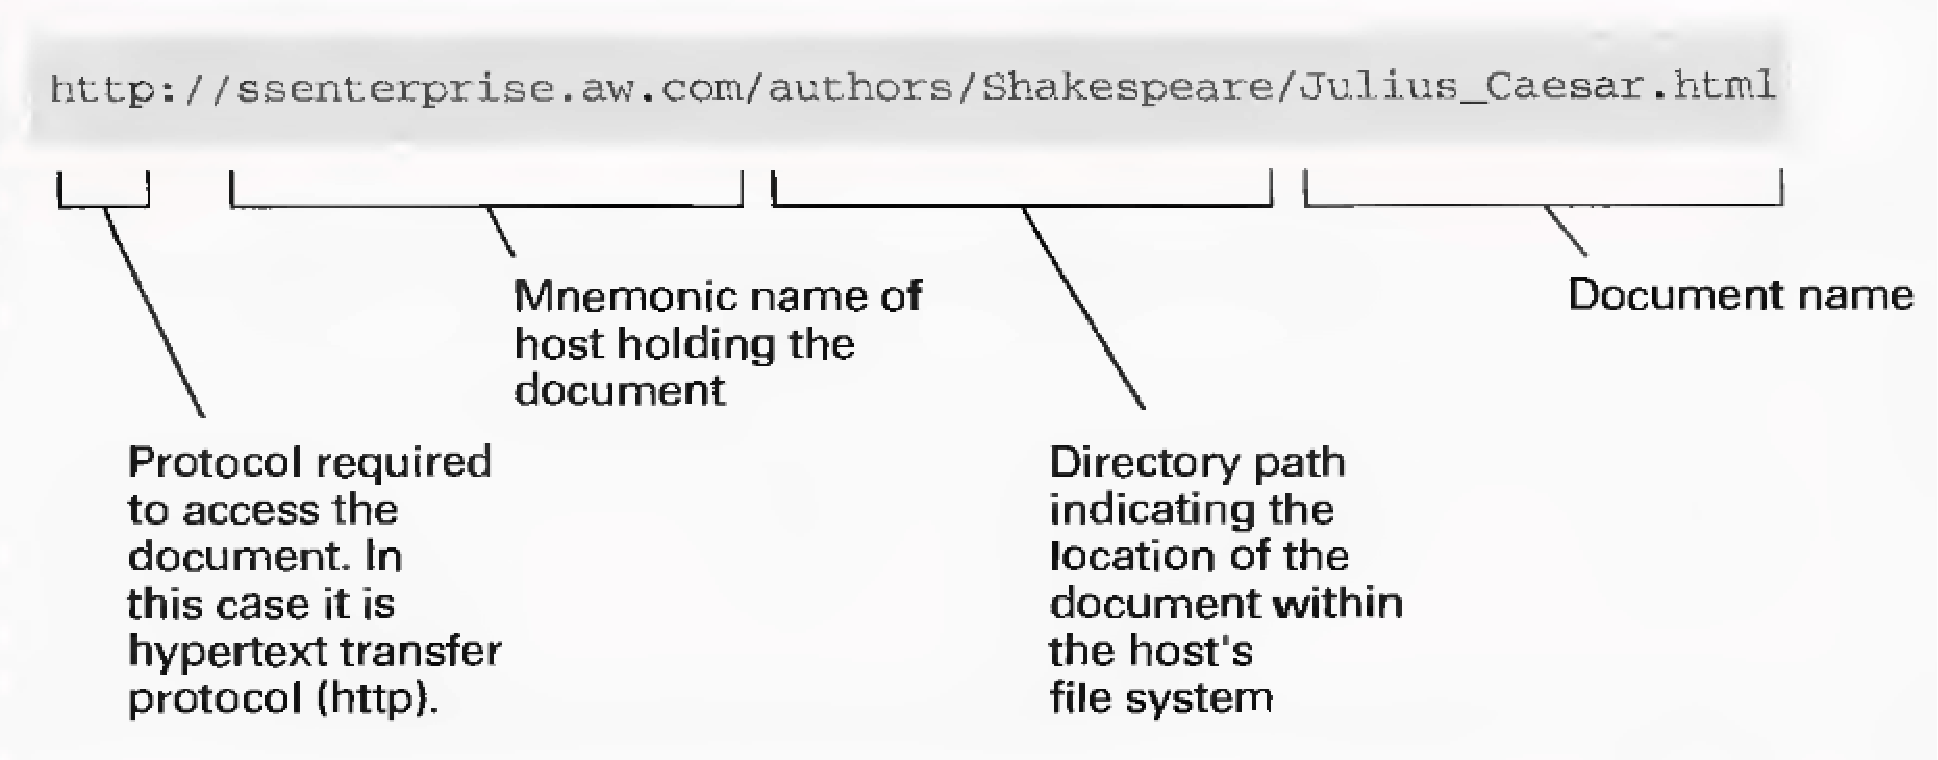
\includegraphics{ch5/fig48.pdf}}
  \caption{Một URL đặc trưng}
  \label{fig:fig4.8}
\end{figure}

Một URL đặc trưng được biểu diễn qua Hình~\ref{fig:fig4.8}. Nó bao gồm bốn phần: giao thức
được sử dụng để giao tiếp với ứng dụng trên máy chủ điều khiển truy cập tới tài liệu, địa
chỉ dễ nhớ của máy tính chứa ứng dụng chủ, đường dẫn cần cho ứng dụng chủ tìm tới thư mục
chứa tài liệu, và cuối cùng là tên của tài liệu. Nói một cách ngắn gọn, URL trong
Hình~\ref{fig:fig4.8} chỉ ra rằng một trình duyệt liên lạc tới một ứng dụng phục vụ Web
đặt trên một máy tính được biết đến là \url{ssenterprise.aw.com} sử dụng giao thức HTTP để
thu nạp tài liệu tên là \texttt{Julius\_Caesar.html} được đặt trong thư mục con
\texttt{Shakespeare} trong thư mục \texttt{authors}.

Đôi khi một URL có thể không nhất thiết phải chứa đủ cả các thành phần được chỉ ra trong
Hình~\ref{fig:fig4.8}. Ví dụ, nếu ứng dụng chủ không cần phải lần theo một đường dẫn thư
mục tới tài liệu, khi đó sẽ không có đường dẫn xuất hiện trong URL nữa. Ngoài ra, đôi khi
một URL sẽ bao gồm chỉ một giao thức và địa chỉ dễ nhớ của một máy tính. Trong trường hợp
này, ứng dụng phục vụ Web tại máy tính đó sẽ trả về một tài liệu được chỉ định trước,
thông thường được gọi là trang chủ (home page), mà thường mô tả thông tin sẵn có trên
website đó. Những URL được làm ngắn gọn như vậy cung cấp một cách thức đơn giản để liên
lạc được với các tổ chức. Ví dụ, URL \url{http://www.aw.com} sẽ dẫn tới trang chủ của Nhà
xuất bản~Addison-Wesley, mà trên đó có chứa các siêu liên kết tới rất nhiều các tài liệu
khác liên quan đến nhà xuất bản và các sản phẩm của họ.

Nhằm đơn giản hóa việc định vị các website, rất nhiều trình duyệt mặc định hiểu rằng giao
thức HTTP sẽ được sử dụng nếu không có giao thức nào được chỉ định. Những trình duyệt này
có thể nạp chính xác trang chủ của Addison-Wesley khi nhận được yêu cầu nạp từ ``URL'' bao
gồm chỉ đơn thuần là \url{www.aw.com}.

Tất nhiên, một người sử dụng Web có thể cần phải tìm kiếm về một chủ đề nào đó hơn là truy
nạp một tài liệu cụ thể. Với mục đích này, rất nhiều website (bao gồm cả các trang chủ của
hầu hết các ISP) cung cấp các dịch vụ của một phương tiện tìm kiếm. Một \textbf{phương
  tiện tìm kiếm} là một gói phần mềm được thiết kế nhằm trợ giúp cho người sử dụng Web xác
định các tài liệu liên quan tới các chủ đề khác nhau. Để sử dụng một phương tiện tìm kiếm,
người sử dụng cần gõ một tập các từ hay cụm từ mà tài liệu mong muốn tìm được có thể chứa
chúng, sau đó phương tiện tìm kiếm sẽ quét toàn bộ các bản ghi của nó, đưa ra báo cáo về
các tài liệu mà nội dung có chứa văn bản cần xác định. Việc cải tiến công nghệ cho các
phương tiện tìm kiếm, bao gồm những phương pháp tốt hơn cho việc xác định các tài liệu
liên quan và cải tiến những hệ thống xây dựng và lưu trữ những bản ghi nằm trong hệ thống
tìm kiếm, đang là một quá trình tiếp diễn.


\begin{figure}[t]
  \begin{quotation}
    \noindent
    \textbf{World Wide Web Consortium} \vspace{0.3cm}
    \\
    The World Wide Web Consortium (W3C) được hình thành vào năm 1994 nhằm đẩy mạnh World
    Wide Web bằng cách phát triển các quy ước chuẩn (được biết đến là các chuẩn W3C). Trụ
    sở W3C được đặt tại CERN, phòng thí nghiệm vật lý hạt nhân năng lượng cao tại Geneva,
    Thụy Sĩ. CERN là nơi mà ngôn ngữ đánh dấu HTML gốc được phát triển theo giao thức HTTP
    nhằm truyền tải các tài liệu HTML qua mạng Internet. Ngày nay W3C là nguồn gốc của rất
    nhiều chuẩn (bao gồm cả những chuẩn cho XML và rất nhiều các ứng dụng đa phương tiện)
    mà có thể tương thích trên diện rộng của những sản phẩm Internet. Bạn có thể nghiên
    cứu thêm về W3C thông qua địa chỉ website của nó tại \url{http://www.w3c.org}
  \end{quotation}
\end{figure}

\subsection*{HTML}
Một tài liệu siêu văn bản truyền thống cũng tương tự như một tệp văn bản vì văn bản của nó
được mã hóa ký tự qua các ký tự sử dụng một hệ thống bảng mã như ASCII hay Unicode. Sự
khác biệt là một tài liệu siêu văn bản có thể chứa các ký tự đặc biệt, gọi là các
\textbf{thẻ} (tag), mà mô tả tài liệu đó xuất hiện trên màn hình hiển thị như thế nào, các
tài nguyên đa phương tiện (như các hình ảnh) đi kèm với tài liệu là gì, và các mục nằm bên
trong tài liệu đó được liên kết tới những tài liệu khác ra sao. Hệ thống các thẻ này được
biết đến là \textbf{Ngôn ngữ Đánh dấu Siêu văn bản (HTML)} (HTML: Hypertext Markup
Language).

Theo cách thức đó, nó chính là thể hiện dưới dạng HTML mà tác giả của một trang Web mô tả
thông tin một trình duyệt cần có để trình diễn trang đó lên màn hình của người sử dụng
và tìm ra bất kỳ tài liệu nào có liên quan đến trang hiện tại. Quá trình này tương tự như
việc thêm các quy định xếp chữ vào một văn bản được gõ trơn (plain text) (có thể sử dụng
một bút màu đỏ) mà một máy xếp chữ sẽ biết được làm thế nào mà các tài liệu có thể xuất
hiện theo một định dạng cuối cùng. Trong trường hợp của siêu văn bản, việc đánh dấu đỏ
được thay thế bằng các thẻ HTML, và một trình duyệt đơn giản là đóng vai trò của máy xếp
chữ, đọc các thẻ HTML nhằm nhận biết được làm thế nào để cho văn bản được trình diễn lên
màn hình máy tính.

\begin{figure} 
  \centering \scalebox{0.5}{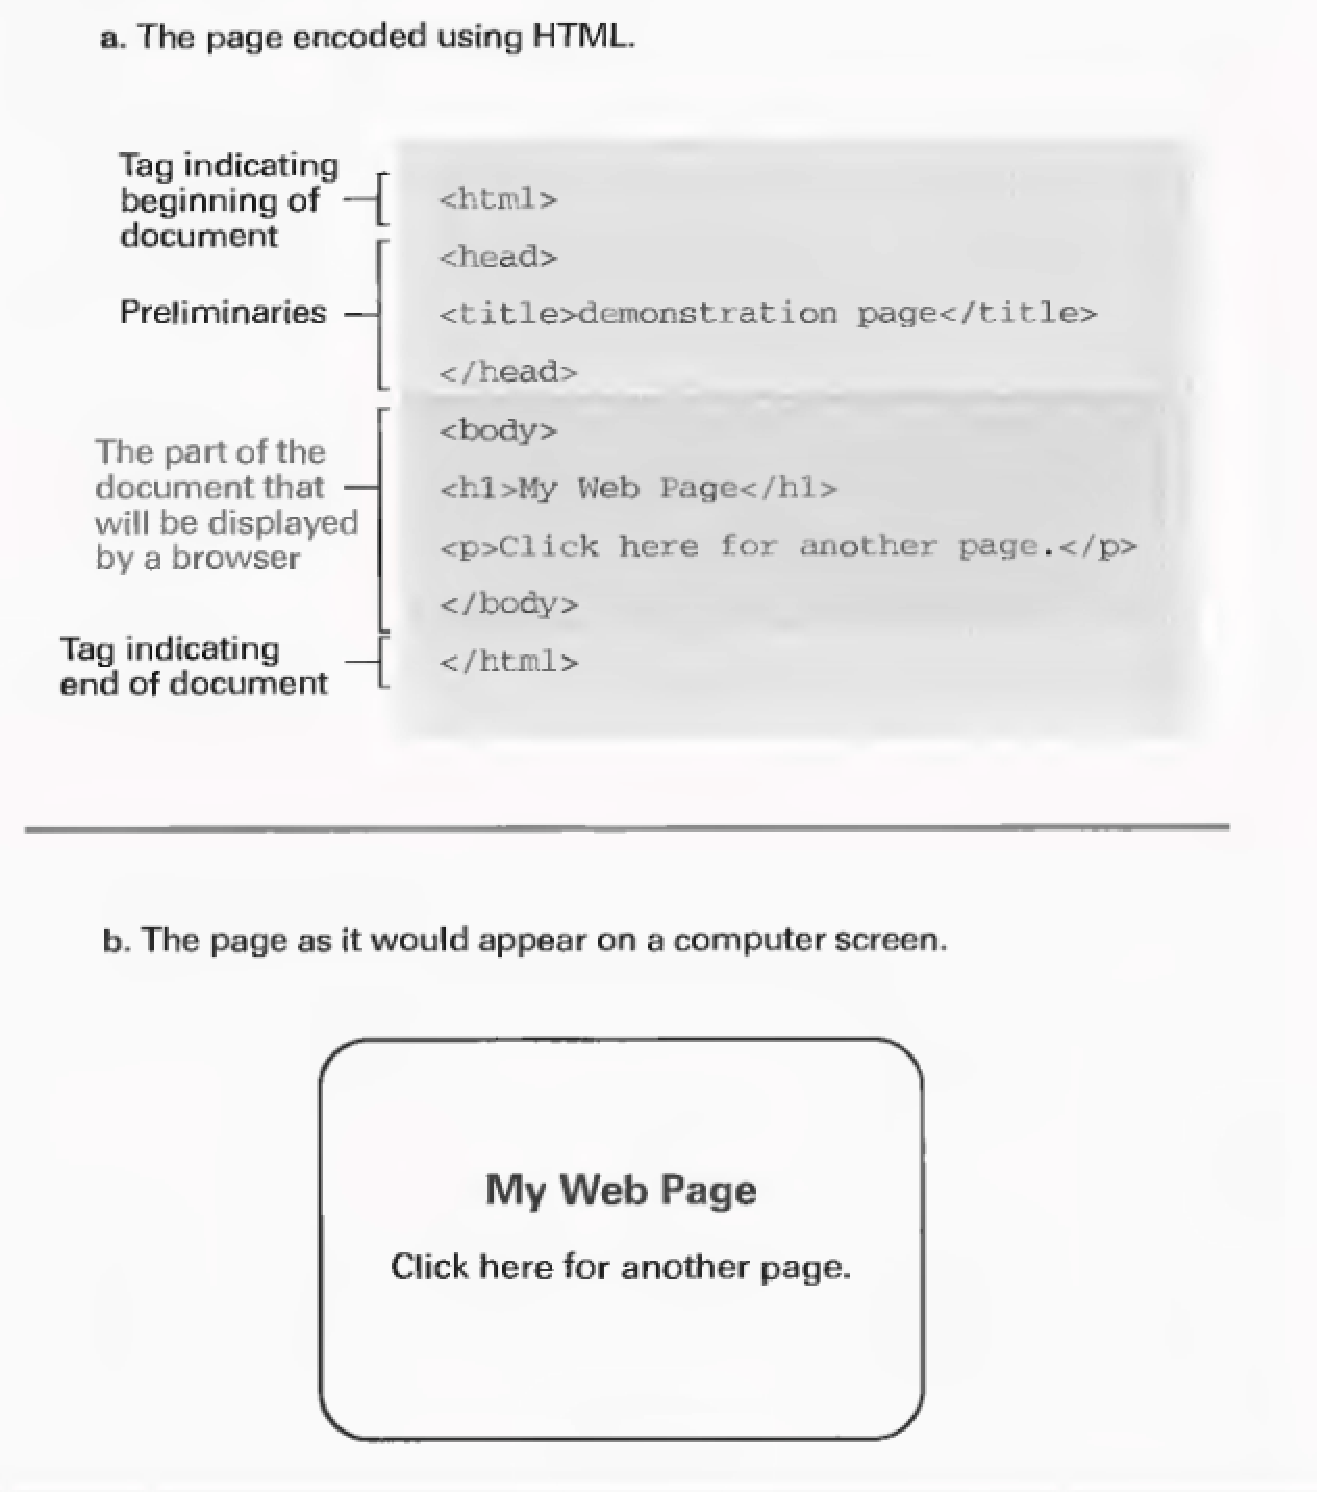
\includegraphics{ch5/fig49.pdf}}
  \caption{Một trang Web đơn giản}
  \label{fig:fig4.9}
\end{figure}

Bản HTML được mã hóa (gọi là bản nguồn) của một trang Web cực kỳ đơn giản được chỉ ra
trong Hình~\ref{fig:fig4.9}a. Cần chú ý rằng các thẻ được phác họa qua các ký tự
\texttt{<} và \texttt{>}.  Tài liệu HTML nguồn bao gồm hai phần--phần đầu (được bao quanh
bởi cặp thẻ \texttt{<head>} và \texttt{</head>}) và phần thân (được bao quanh bởi cặp thẻ
\texttt{<body>} và \texttt{</body>}). Sự khác biệt giữa phần đầu và phần thân của một
trang Web tương tự như phần đầu và phần thân của một cuốn sổ ghi nhớ trong nội bộ một tổ
chức. Trong cả hai trường hợp, phần đầu thường chứa thông tin sơ bộ về tài liệu (ngày,
tiêu đề,… trong trường hợp của sổ ghi nhớ). Phần thân chứa nội dung cốt lõi của tài liệu,
mà trong trường hợp của trang web thì đó là các tài liệu được trình chiếu trên màn hình
máy tính khi trang đó được hiển thị lên.

Phần đầu của trang Web hiển thị trong Hình~\ref{fig:fig4.9}a chứa chỉ duy nhất tiêu đề của
tài liệu (được bao quanh bởi cặp thẻ ``title''). Tiêu đề này chỉ có mang tính chất là dẫn
chứng cho tài liệu; nó không phải là phần được hiển thị lên trên màn hình máy tính. Nội
dung mà sẽ hiển thị lên trên màn hình máy tính được chứa trong phần thân của tài liệu.


Mục đầu tiên trong phần thân của tài liệu trong Hình~\ref{fig:fig4.9}a là tiêu đề cấp độ 1
(được bao quanh bởi cặp thẻ \texttt{<h1>} và \texttt{</h1>}) chứa dòng văn bản ``My Web
Page.''. Là tiêu đề cấp độ 1 có nghĩa là trình duyệt sẽ hiển thị văn bản này nổi bật trên
màn hình. Mục tiếp theo trong phần thân là một đoạn văn bản (được bao quanh bởi cặp thẻ
\texttt{<p>} và \texttt{</p>}) chứa đoạn văn bản ``Click here for another
page.''. Hình~\ref{fig:fig4.9}b chỉ ra trang web sẽ được hiển thị như thế nào trên màn
hình máy tính thông qua một trình duyệt.

Trong hình dạng hiện tại của nó, trang Web trong Hình~\ref{fig:fig4.9} không có đầy đủ các
chức năng nên khi đó sẽ không có gì xảy ra khi người xem kích chuột vào từ \textit{here},
 mặc dù theo yêu cầu trình duyệt sẽ phải hiển thị một trang khác. Để đạt được yêu cầu, ta cần phải liên kết từ \textit{here} tới một tài liệu khác.

\begin{figure}
  \centering \scalebox{0.5}{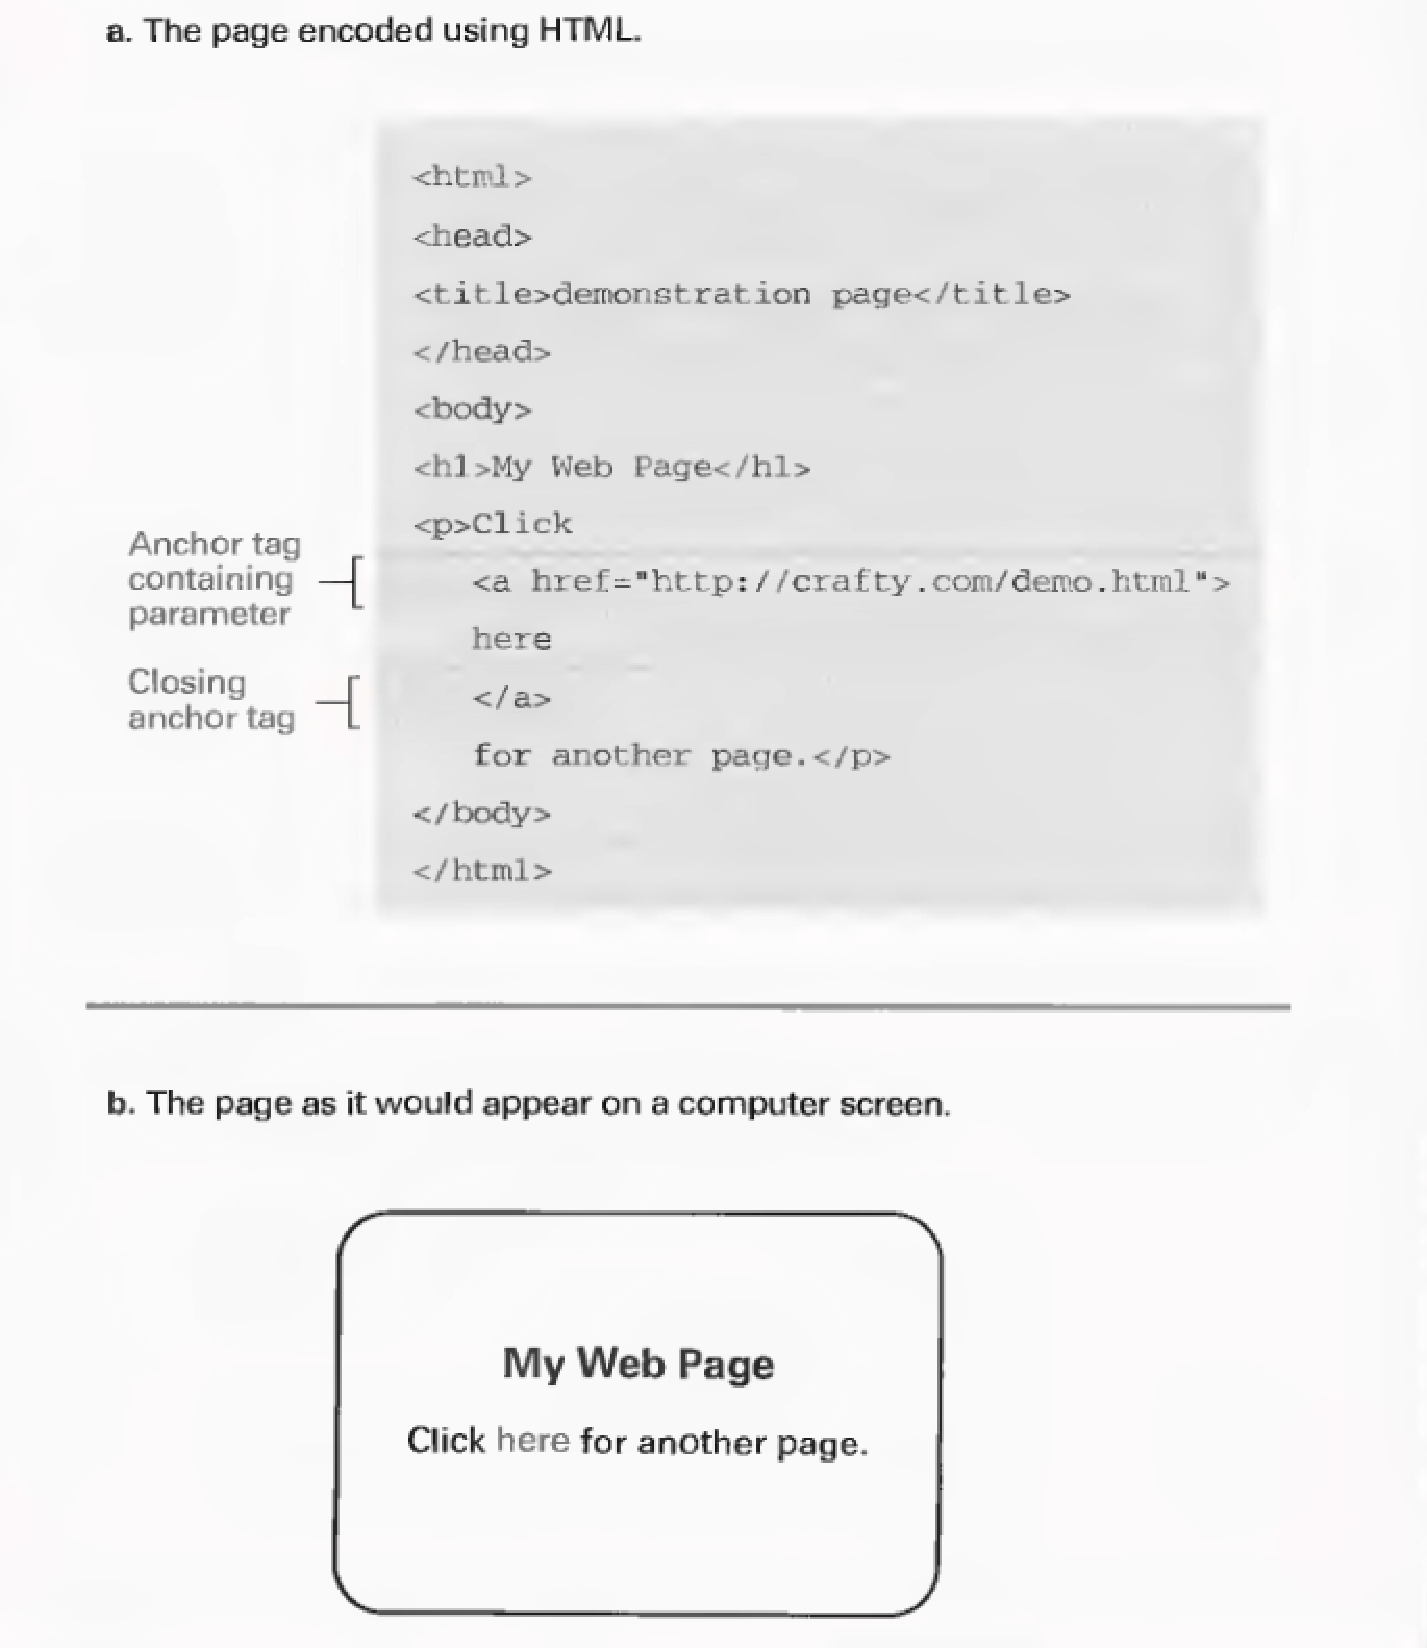
\includegraphics{ch5/fig410.pdf}}
  \caption{Một trang Web mở rộng}
  \label{fig:fig4.10}
\end{figure}

Ta giả sử rằng khi từ here được kích chuột vào, ta muốn trình duyệt truy lục và hiển thị
trang web tại URL \url{http://crafty.com/demo.html}. Để làm được điều đó, trước tiên ta
phải bao quanh từ \texttt{here} trong bản nguồn của trang bằng cặp thẻ \texttt{<a>} và
\texttt{</a>}, cặp thẻ này được gọi là thẻ mấu neo. Bên trong thẻ mở mấu neo, ta chèn thêm
tham số \texttt{href= “http://crafty.com/demo.html”} (như trong Hình~\ref{fig:fig4.10}a)
với mục đích chỉ ra siêu văn bản tham chiếu (href: hypertext reference) kết hợp với thẻ
trong URL ngay sau dấu bằng (\url{http://crafty.com/demo.html})

Khi có thêm các thẻ mấu neo, trang Web bây giờ sẽ hiển thị trên màn hình máy tính như
trong Hình~\ref{fig:fig4.10}b. Chú ý rằng sự hiển thị này tương tự như trong
Hình~\ref{fig:fig4.9}b ngoại trừ từ \textit{here} được làm cho nổi bật bằng mầu sắc, điều
đó chỉ ra rằng nó là một liên kết tới một tài liệu Web khác. Việc kích chuột vào những cụm
từ nổi bật như vậy sẽ khiến cho trình duyệt truy lục và hiển thị tài liệu Web kết hợp
trong liên kết đó. Chính vì vậy thông qua các thẻ mấu neo mà các tài liệu Web được liên
kết tới những tài liệu khác.

Cuối cùng, ta cũng cần phải được nói sơ qua làm thế nào để một hình ảnh có thể được
hiển thị trên một trang Web đơn giản. Với ý định này, giả sử rằng một ảnh mã hóa theo định
dạng JPEG mà ta muốn chèn vào được lưu trữ trong cùng thư mục với bản nguồn HTML của
trang Web trên site chủ HTTP. Ngoài ra, ta cũng giả sử rằng tên của tệp ảnh đó là
\texttt{OurImage.jpg}. Với những điều kiện như vậy, ta có thể ra chỉ thị cho một
trình duyệt hiển thị ảnh đó trên đầu của trang Web bằng cách chèn vào thêm thẻ hình ảnh
(img) \texttt{<img src = "OurImage.jpg">} ngay sau thẻ \texttt{<body>} trong tài liệu
nguồn HTML. Điều này diễn đạt cho trình duyệt hiểu là một ảnh có tên là
\texttt{OurImage.jpg} có thể được hiển thị tại vị trí đầu tiên của tài liệu. (Ký hiệu
\texttt{src} là dạng viết ngắn gọn của từ ``source'', có nghĩa là thông tin đằng sau dấu
bằng chỉ ra đường dẫn tới tệp hình ảnh mà sẽ được hiển thị.) Khi trình duyệt tìm thấy thẻ
này, nó sẽ gửi một thông điệp ngược trở về ứng dụng chủ HTTP mà từ đó, ứng dụng chủ sẽ
nhận được yêu cầu của tài liệu gốc tới tệp hình ảnh \texttt{OurImage.jpg} và sau đó trình
duyệt sẽ hiển thị hình ảnh một cách thích hợp.

Nếu ta di chuyển thẻ hình ảnh tới cuối cùng của tài liệu, ngay trước thẻ
\texttt{</body>}, khi đó trình duyệt sẽ hiển thị hình ảnh tại vị trí cuối cùng của trang
Web. Tất nhiên, có nhiều kỹ thuật phức tạp hơn cho việc đặt vị trí của một hình ảnh trên
một trang Web, nhưng chúng không nhất thiết phải được đề cập tới ở đây.

\subsection*{XML}

HTML về cơ bản là một hệ thống ký hiệu mà qua đó một tài liệu văn bản với việc hiển thị
của tài liệu đó có thể được mã hóa như là một tệp văn bản đơn giản. Theo cách thức tương
tự thì ta cũng có thể mã hóa một tài liệu không còn là nguyên bản như những tệp văn
bản--một ví dụ là về các bản nhạc. Khi lưu trữ thông tin về một mẫu khuông nhạc, các đường
gạch nhịp và nốt trong đó âm nhạc được miêu tả theo cách truyền thống không được thể hiện
theo định dạng từng ký tự một của những tệp văn bản. Tuy nhiên, ta có thể khắc phục
được vấn đề này bằng cách phát triển một hệ thống ký hiệu thay thế. Nói một cách chính xác
hơn, ta có thể thỏa thuận trình bày bắt đầu của khuông nhạc bằng thẻ \texttt{<staff
  clef = ``treble''>}, kết thúc một khuông nhạc bằng thẻ \texttt{</staff>}, trình bày ký
hiệu nhịp theo dạng \texttt{<time> 2/4 </time>}, thẻ bắt đầu và kết thúc của một nhịp là
\texttt{<measure>} và \texttt{</measure>}, và theo một thứ tự định sẵn thì một nốt như nốt
thứ tám trên điệu thứ C được ký hiệu là \texttt{<notes>eight C</notes>},… Khi đó, đoạn văn
bản sau:
\begin{verbatim}
      <staff clef = "treble">
           <key>C minor</key>
           <time> 2/4 </time>
           <measure> 
               <rest> egth </rest> 
               <notes> egth G, egth G, egth G </notes>
           </measure>
           <measure> 
               <notes> hlf E </notes>
           </measure>
      </staff>
\end{verbatim}
có thể được sử dụng để mã hóa bản nhạc chỉ ra trong Hình~\ref{fig:fig4.11}.

\begin{figure}[bt] 
  \centering \scalebox{0.4}{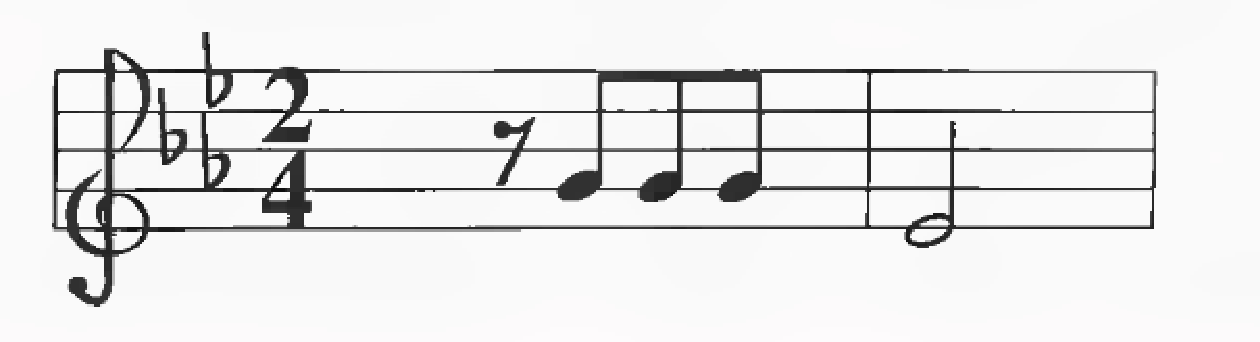
\includegraphics{ch5/fig411.pdf}}
  \caption{Hai khuông đầu tiên trong bản Symphony thứ năm của Beethoven}
  \label{fig:fig4.11}
\end{figure}


Bằng việc sử dụng những ký hiệu như vậy, một bản nhạc có thể được mã hóa, sửa đổi, lưu trữ
và truyền qua mạng Internet như những tệp văn bản. Hơn nữa, phần mềm có thể được viết ra
nhằm trình diễn nội dung của những tệp văn bản như vậy theo một khuôn dạng âm nhạc truyền
thống hay thậm chí có thể chơi được bản nhạc đó trên một nhạc cụ điện tử.

Chú ý rằng hệ thống mã hóa bản nhạc của ta bao gồm khuôn dạng tương tự được sử dụng bởi
ngôn ngữ HTML. Ta đã lựa chọn cách thức ký hiệu những thẻ nhận dạng các thành phần bởi cặp
ký tự \texttt{<} và \texttt{>}. Ta cũng quyết định chỉ ra điểm bắt đầu và kết thúc của
những cấu trúc đó (ví dụ như một khuông nhạc, một chuỗi các nốt nhạc, hay một nhịp nhạc)
bởi những thẻ có tên trùng nhau-–thẻ kết thúc được ký hiệu thêm một ký tự \texttt{/} (thẻ
\texttt{<measure>} được kết thúc bằng thẻ \texttt{</measure>)}. Và ta cũng đã quyết định
chỉ ra những thuộc tính đặc biệt bên trong các thẻ bằng các biểu thức như \texttt{clef =
  “treble”}. Khuôn dạng tương tự này có thể cũng được sử dụng để phát triển các hệ thống
mô tả những định dạng khác như các biểu thức toán học hay đồ họa.

Ngôn ngữ \textbf{đánh dấu mở rộng} (XML: Extensible Markup Language) là một khuôn dạng
được chuẩn hóa (tương tự như ví dụ về bản nhạc của ta) cho việc thiết kế những hệ
thống ký hiệu cho việc hiển thị những dữ liệu dạng như các tệp văn bản. (Trên thực tế, XML
là một ngôn ngữ dẫn xuất được làm đơn giản hóa từ một tập các chuẩn cũ hơn gọi là Standard
Generalized Markup Language, với ký hiệu viết tắt là SGML.)  Theo như chuẩn XML, những hệ
thống ký hiệu với tên gọi là \textbf{ngôn ngữ đánh dấu} được phát triển cho việc mô tả
toán học, trình diễn đa phương tiện, và âm nhạc. Nói tóm lại, HTML là ngôn ngữ đánh dấu
dựa trên chuẩn XML mà được phát triển nhằm hiển thị các trang Web. (Thực tế là phiên bản
gốc của HTML được phát triển trước chuẩn XML đã được làm cho vững chắc, và do đó một vài
tính năng của HTML không thích ứng hoàn toàn với XML. Điều này cũng giải thích vì sao bạn
có thể đã thấy những tham khảo về XHTML, đó là một phiên bản của HTML với một sự kết hợp
khá chặt chẽ với XML.)

XML cung cấp một tiền lệ tốt cho việc làm thế nào mà các chuẩn được thiết kế được ứng dụng
trong phạm vi rộng. Đúng hơn là với những ngôn ngữ đánh dấu không liên quan cho việc mã
hóa rất nhiều dạng tài liệu, việc thiết kế một cách độc đáo phương pháp biểu diễn bằng XML
là nhằm phát triển một chuẩn chung cho các ngôn ngữ đánh dấu khác. Với chuẩn này, những
ngôn ngữ đánh dấu có thể được khai thác trong rất nhiều các ứng dụng. Những ngôn ngữ đánh
dấu được phát triển theo cách thức này đều có một tính chất giống nhau mà cho phép chúng
kết hợp với nhau nhằm thu được những ngôn ngữ đánh dấu dùng cho những ứng dụng phức tạp
như những tài liệu văn bản chứa các phân đoạn của một bản nhạc và các biểu thức toán học.

Cuối cùng ta cũng cần phải chú ý rằng XML công nhận sự phát triển của những ngôn ngữ
đánh dấu mới khác so với HTML mà trong đó chúng có mục đích là làm nổi bật ngữ nghĩa hơn
là việc hiển thị. Ví dụ, với HTML các thành phần (ingredient) trong một công thức làm món
ăn có thể được đánh dấu sao cho chúng xuất hiện như là một danh sách mà trong đó mỗi thành
phần được đặt trên một dòng riêng biệt. Nhưng nếu ta sử dụng các thẻ định hướng có
ngữ nghĩa (semantic-oriented), các thành phần trong công thức đó có thể được đánh dấu dưới
dạng như những thành phần hợp thành tổng quát (có thể chỉ sử dụng các thẻ như
\texttt{<ingredient>} và \texttt{</ingredient>}) hơn là các mục chọn đơn thuần trong một
danh sách. Sự khác biệt ở đây tuy là rất nhỏ nhưng lại khá quan trọng. Cách tiếp cận theo
hướng có ngữ nghĩa sẽ cho phép các công cụ tìm kiếm có thể xác định những công thức món ăn
chứa hay không chứa những thành phần nào đó, đây sẽ là một cải tiến đáng kể vượt qua tình
trạng hiện tại của đề tài nghiên cứu mà trong đó chỉ những công thức chứa hay không chứa
những từ cụ thể mới được xác định. Nói một cách chính xác hơn, nếu các thẻ có ngữ nghĩa
được sử dụng, một công cụ tìm kiếm có thể xác định công thức cho món lasagna không chứa
rau bina (spinach), trong khi đó một cách thức tìm kiếm dựa vào chỉ đơn thuần là nội dung
của từ sẽ bỏ qua một công thức mà bắt đầu bằng câu ``This lasagna does not contain
spinach.'' Tóm lại, bằng việc sử dụng một chuẩn có phạm vi trên mạng Internet cho việc
đánh dấu các tài liệu theo hướng có ngữ nghĩa hơn là việc hiển thị, một Web \textit{ngữ
  nghĩa} phạm vi toàn cầu (World Wide Semantic Web) có thể sẽ được tạo ra thay thế cho Web
cú pháp phạm vi toàn cầu (World Wide Syntactic Web) mà ta đang có hiện nay.

\subsection*{Các hoạt động phía client và phía server}

Bây giờ ta xem xét các bước được yêu cầu đối với một trình duyệt để có thể truy nạp
được trang Web đơn giản đã chỉ ra trong Hình~\ref{fig:fig4.10} và hiển thị nó lên màn hình
máy tính qua trình duyệt. Trước tiên, đóng vai trò của một ứng dụng khách, trình duyệt sẽ
sử dụng thông tin có được trong URL (có thể nhận được từ người sử dụng trình duyệt) để
liên lạc tới ứng dụng phục vụ Web, điều khiển truy cập tới trang Web và yêu cầu một bản
sao của trang Web cần phải được truyền tới ứng dụng khách. Ứng dụng chủ sẽ đáp lại yêu cầu
bằng cách gửi tài liệu văn bản được hiển thị trong Hình~\ref{fig:fig4.10}a đến trình
duyệt. Trình duyệt sau đó sẽ dịch các thẻ HTML có trong tài liệu nhằm xác định trang Web
đó cần được hiển thị như thế nào và trình diễn tài liệu đó trên màn hình máy tính của
trình duyệt một cách phù hợp. Người sử dụng trình duyệt sẽ nhìn thấy một hình ảnh như được
mô tả trong Hình~\ref{fig:fig4.10}b. Nếu người dùng sau đó kích chuột vào từ
\textit{here}, trình duyệt sẽ sử dụng URL trong thẻ mấu neo kết hợp trong đó để liên lạc
tới ứng dụng chủ tương ứng nhằm thu nạp và hiển thị một trang Web khác. Nói tóm lại, quá
trình này bao gồm chỉ đơn thuần là thao tác lấy và hiển thị các trang Web một cách trực
tiếp bởi người dùng.

Nhưng nếu ta muốn một trang Web trong đó bao gồm cả hoạt ảnh (animation) hay một
trang Web cho phép khách hàng điền đầy đủ những thông tin vào một đơn đặt hàng và gửi đơn
đặt hàng đó đi? Những thứ đó cần phải yêu cầu hoạt động bổ trợ từ trình duyệt hay ứng dụng
phục vụ Web. Những hoạt động như vậy được gọi là những hoạt động \textbf{phía client}
(client-side) nếu chúng được thực hiện bởi một ứng dụng khách (ví dụ như một trình duyệt)
hay \textbf{phía server} (server-side) nếu chúng được thực hiện bởi một ứng dụng phục vụ
(ví dụ như ứng dụng phục vụ Web).

Hoạt ảnh trên một trang Web thông thường là một hoạt động phía client. Thông tin cần có
cho hoạt ảnh được truyền tới trình duyệt cùng với văn bản có trong trang Web. Sau đó hoạt
ảnh mới được thực thi dưới sự điều khiển của trình duyệt.

Ngược lại, giả sử một đại lý du lịch yêu cầu các khách hàng cần phải xác định đích đến
mong muốn và ngày du lịch, khi đó đại lý sẽ trình chiếu cho khách hàng một trang Web đã
được tùy biến chỉ chứa thông tin thích hợp với nhu cầu của khách hàng. Trong trường hợp
này, website của đại lý du lịch trước tiên sẽ cung cấp một trang Web và được hiển thị cho
một khách hàng với những đích đến có thể. Dựa trên những thông tin cơ bản này, khách hàng
sẽ chỉ ra những đích đến yêu thích và những ngày du lịch mà họ mong muốn (một hoạt động
phía client). Thông tin này sau đó sẽ được truyền về ứng dụng chủ của đại lý nơi mà nó sẽ
được dùng để tạo dựng một trang Web tương ứng đã được tùy biến (một hoạt động phía server)
và sau đó sẽ được gửi tới trình duyệt của khách hàng.

Một ví dụ tương tự xảy ra trong trường hợp một người sử dụng những dịch vụ của một công cụ
tìm kiếm. Ở đây, người này chỉ ra một chủ đề ưa thích (một hoạt động phía client) mà sau
đó được truyền tới công cụ tìm kiếm, nơi mà một trang Web được tùy biến xác định những tài
liệu nào có thể phù hợp được tạo dựng (một hoạt động phía server) và gửi trả về cho ứng
dụng khách.

Có rất nhiều hệ thống thực hiện các hoạt động phía client và phía server, mỗi hệ thống đều
cạnh tranh với hệ thống khác bằng những tính năng nổi bật của mình. Có một cách thức điều
khiển các hoạt động phía client tuy đã ra đời từ sớm những vẫn khá phổ biến, đó là việc
triển khai viết các chương trình dưới mã của ngôn ngữ Javascript (được phát triển bởi Công
ty truyền thông Netscape) bên trong tài liệu nguồn HTML của một trang Web. Khi đó, một
trình duyệt có thể bóc tách những chương trình này và thực hiện chúng theo đúng yêu
cầu. Một cách tiếp cận khác (được phát triển bởi Sun Microsystems) là trước tiên truyền
một trang Web tới trình duyệt và sau đó truyền những đơn vị chương trình bổ trợ gọi là
applet (được viết bằng ngôn ngữ Java) tới trình duyệt theo yêu cầu bên trong tài liệu
nguồn HTML. Vẫn còn một cách tiếp cận khác nữa đó là hệ thống Flash (được phát triển bởi
Macromedia), thông qua hệ thống Flash, những trình diễn đa phương tiện trên diện rộng có
thể được triển khai một cách đơn giản.


Một cách thức điều khiển các hoạt động phía server là sử dụng một tập các chuẩn gọi là CGI
(Common Gateway Interface) mà qua đó các ứng dụng khách có thể yêu cầu thực thi các chương
trình được lưu trữ trên một máy chủ. Một biến tố của cách tiếp cận này (được phát triển
bởi Sun Microsystems) là cho phép các ứng dụng khách khiến  những đơn vị chương trình
như servlet được thực thi trên phía ứng dụng chủ. Một phiên bản được đơn giản hóa của cách
tiếp cận servlet có thể được sử dụng khi yêu cầu được gửi tới phía server là việc tạo dựng
một trang Web được tùy biến, như trong ví dụ về đại lý du lịch. Trong trường hợp này, các
mẫu trang Web được gọi là JavaServer Pages (JSP) được lưu trữ tại máy chủ phục vụ Web và
được bổ sung từ những thông tin nhận từ phía một ứng dụng khách nào đó. Một cách tiếp cận
tương tự được sử dụng bởi Microsoft, nơi mà các mẫu từ những trang Web được tùy biến được
tạo dựng ra với tên gọi là Active Server Page (ASP). Ngược lại với những hệ thống đòi hỏi
cần phải có bản quyền, PHP (tiền thân xuất phát từ Personal Home Page nhưng ngày nay được
hiểu với nghĩa mới là PHP Hypertext Processor) là một hệ thống mã nguồn mở cũng rất thích hợp cho việc triển
khai các tính năng phía server.

Cuối cùng, sẽ thật là thiếu sót nếu ta không nhận ra những vấn đề về an ninh và 
quy tắc phát sinh từ việc cho phép những ứng dụng khách và ứng dụng phục vụ thực hiện những
chương trình trên máy tính của người khác. Trên thực thế những ứng dụng phục vụ Web đó
thường truyền tải các chương trình tới phía các ứng dụng khách nơi mà chúng được thực thi
dẫn tới những sự nghi ngờ liên quan đến vấn đề về nội quy trên phía ứng dụng chủ và những
vấn đề về bảo mật trên phía ứng dụng khách. Nếu ứng dụng khách thực thi bất kỳ chương
trình nào một cách mù quáng được gửi tới từ một ứng dụng phục vụ Web, nó có thể mở cửa
chính mình cho các hoạt động nguy hiểm được thực hiện bởi ứng dụng chủ. Tương tự như vậy,
trên thực tế những ứng dụng khách này có thể là nguyên nhân khiến cho các chương trình có
thể được thực thi trên ứng dụng chủ dẫn tới những vấn đề về nội quy trên phía ứng dụng
khách và những vấn đề liên quan đến bảo mật trên phía ứng dụng chủ. Nếu một ứng dụng chủ
nào đó thực hiện một cách mù quáng bất kỳ chương trình nào được gửi tới mình từ một ứng
dụng khách bất kỳ, những lỗ hổng an ninh và sự thiệt hại tiềm năng trên máy chủ có thể sẽ
xảy ra.

\subsection*{Câu hỏi \& Bài tập}

\begin{enumerate}
\item Một URL là gì? Một trình duyệt là gì?
\item Một ngôn ngữ đánh dấu là gì?
\item Sự khác nhau giữa HTML và XML là gì?
\item Mục đích của những thẻ HTML dưới đây là gì?

  \begin{inparaenum}[a.]
  \item \texttt{<html>} \qquad
  \item \texttt{<head>} \qquad
  \item \texttt{</body>} \qquad
  \item \texttt{<fa>}
  \end{inparaenum}

\item Những cụm từ phía client (client-side) và phía server (server-side) đề cập tới vấn
  đề gì?
\end{enumerate}






























%%% Local Variables: 
%%% mode: latex
%%% TeX-master: "../tindaicuong"
%%% End: 
